\section{Data Analysis: Community}
\label{sec:community}

The greenhouse gas emissions from a given \event is in direct proportion to
the average distance traveled by the participants of this \event.
To understand emissions, we must therefore estimate the nature of the
communities that attend each conference. 

The aggregated information we describe below falls into two main categories:
first, the demographic distribution of the participants to the conferences
conditioned by various factors, and second, the participation habits of the
community through recurring participation to a given conference and the
overlap in participation between different conferences.

%% Through this section, we present the results of our data analysis in a
%% neutral way. We point out phenomena that came out as a
%% surprise to us, but defer opinionated observations and practical conclusions to
%% Section~\ref{sec:opinions}.

\subsection{Demographics: Where Did Participants Come From?}
\label{subsec:demo}

\begin{figure}
  \centering
  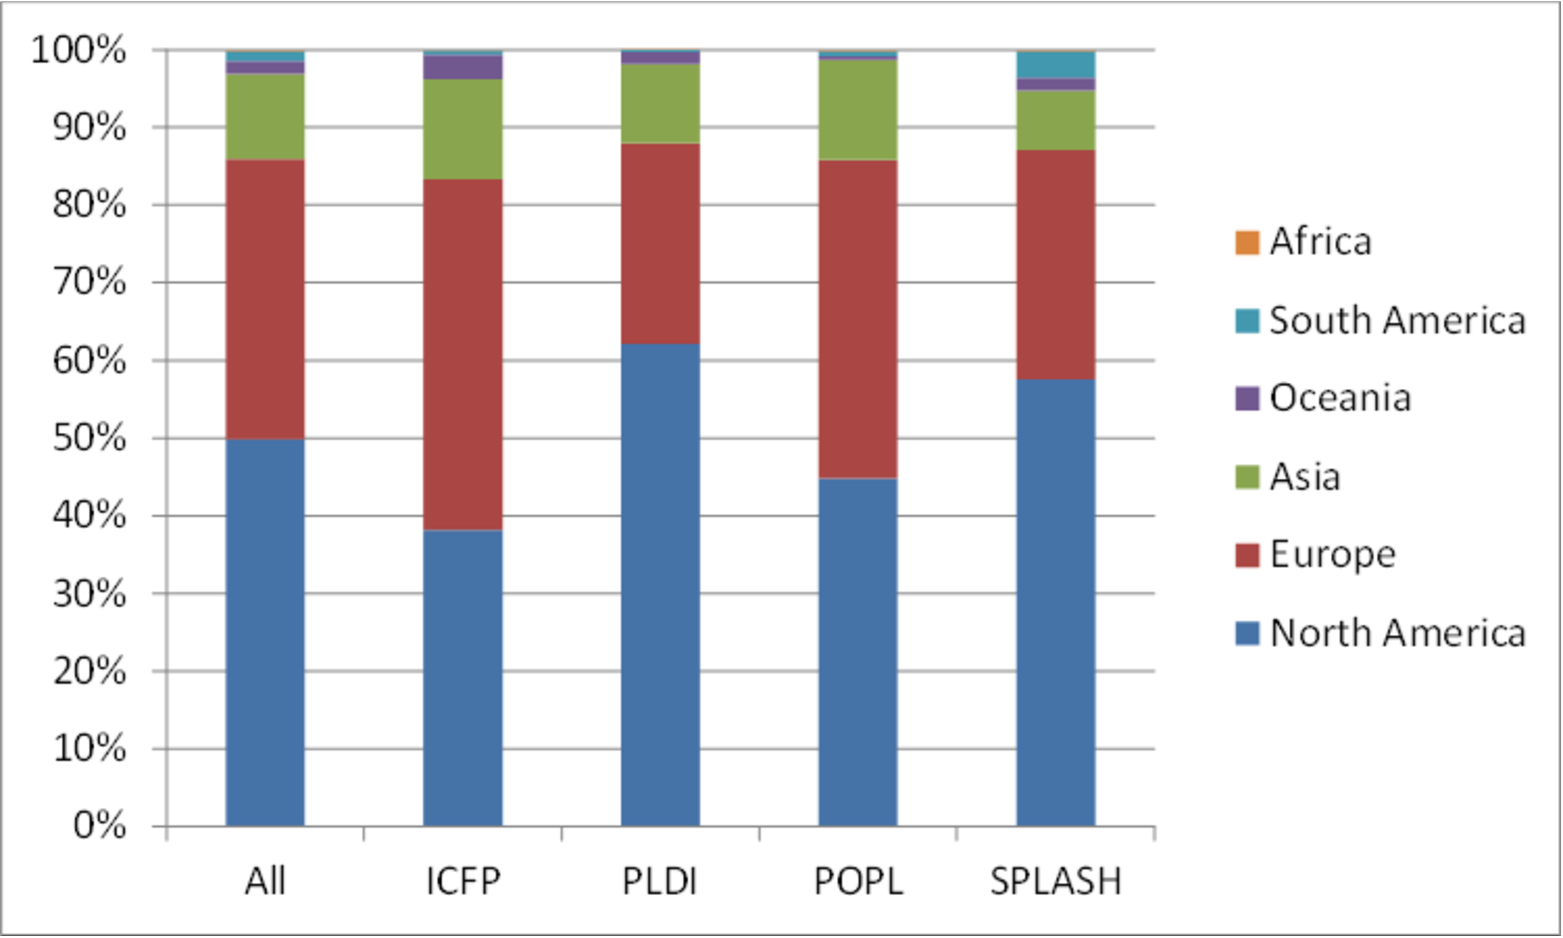
\includegraphics[width=0.7\textwidth]{ParticipantsOrigin.pdf}
  \caption{Overall origin of participants per conference.}
  \label{fig:demo-per-conf}
\end{figure}

\begin{table}
  \csvautotabular{../../output/sigplan/demographic_per_conf.csv}
\caption{For each kind of conference, distribution of participants per continent of origin}
\label{table:demo-per-conf}
\end{table}


Figure~\ref{fig:demo-per-conf}\footnote{The graphical representations in this preliminary draft are based on a slightly different version of our dataset than the one used by our tool. There may be some minor discrepancies between these representations and the raw tables presented.} and Table~\ref{table:demo-per-conf} show
where all participants came from. For each conference, we depict the
distribution of attendance per continent. Table~\ref{table:demo-per-conf}
shows the portion of attendants originating from the same continent as the
one the event took place in. To a first approximation, maximizing this last
metric, i.e. hosting conferences in the continent containing the majority of
its community, is a good thing.

Taken as a whole, these conferences attracted 50\% participants from North
America, 36\% from Europe, 11\% from Asia, 2\% from Oceania, 1\% from South
America, and less than 0.2\% from Africa.
The data also displays some degree of geographical affinity for the 
various conferences.
Notably, PLDI and SPLASH appear to be quite North-America-centric, while
ICFP's core community seems to have a strong anchor in Europe as well.

\begin{table}
  \csvautotabular{../../output/sigplan/demographic.csv}
  \caption{For each \event, continent in which it took place and distribution of
    each continent by origin of participants. The final column indicates the
    portion of participants that traveled from the same continent the
    conference took place in.}
  \label{table:demo-per-event}
\end{table}

\begin{figure}
  \centering
  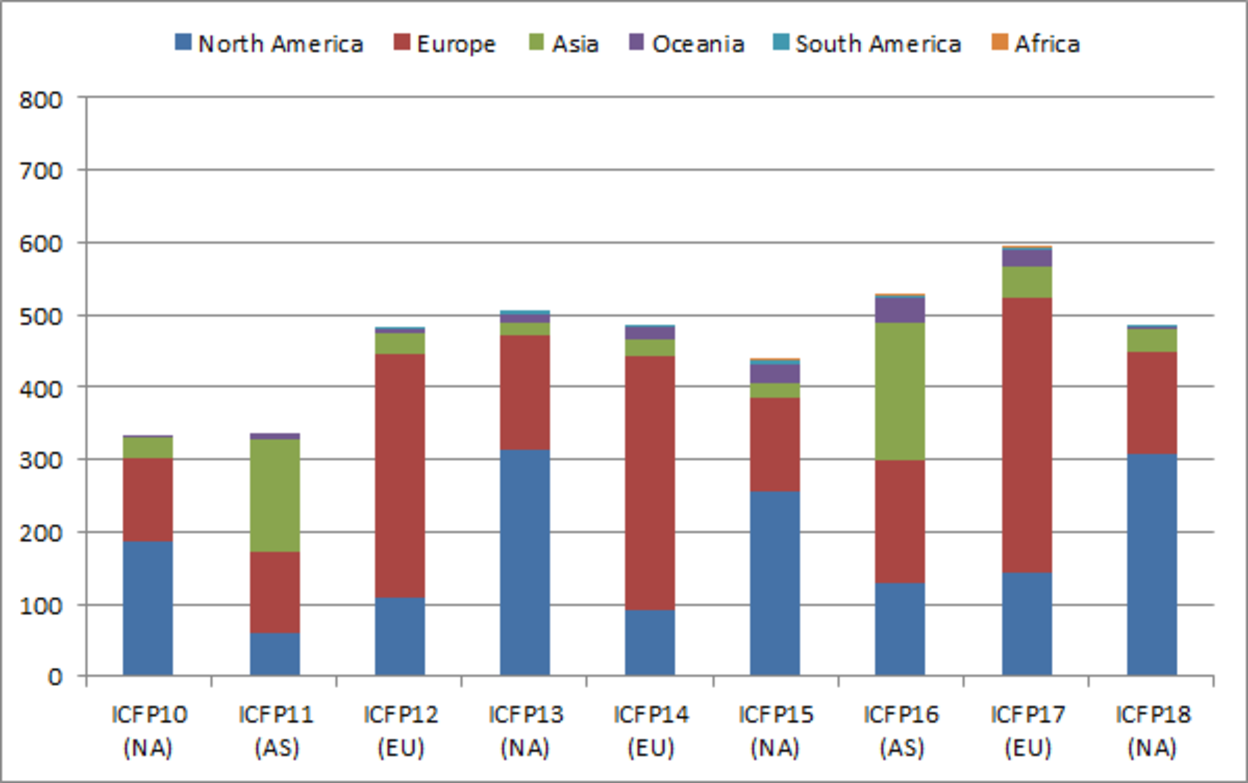
\includegraphics[width=0.45\textwidth,height=1.8in]{ParticipantsOriginICFP.pdf}
  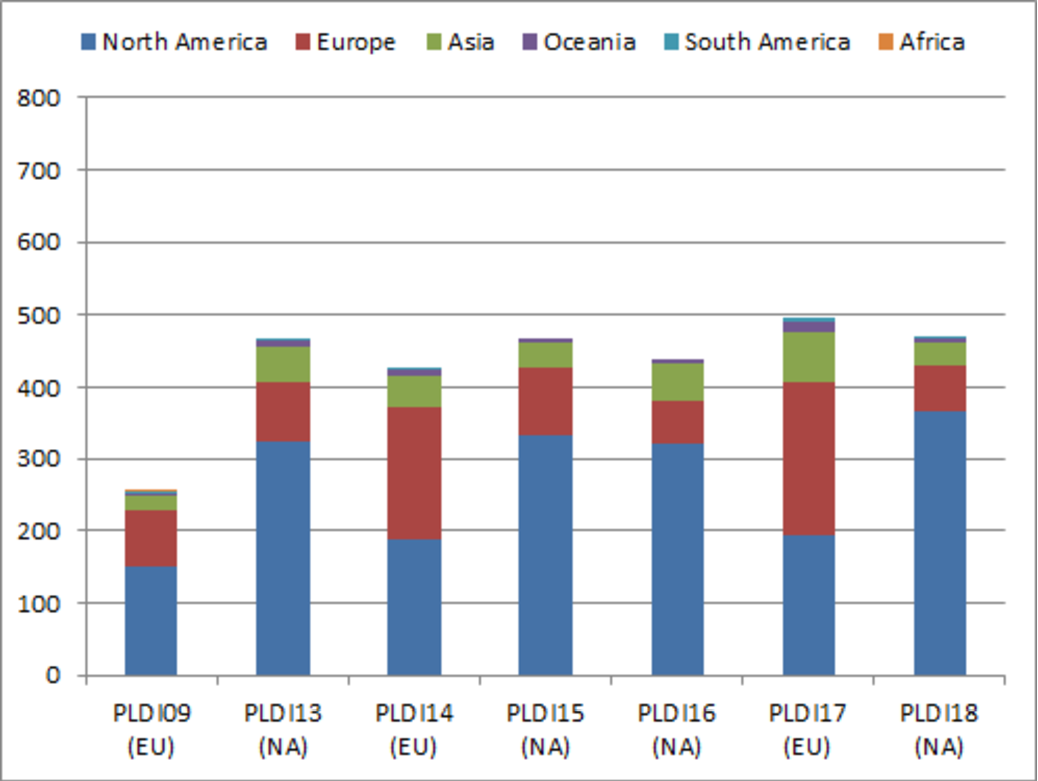
\includegraphics[width=0.45\textwidth,height=1.8in]{ParticipantsOriginPLDI.pdf}
  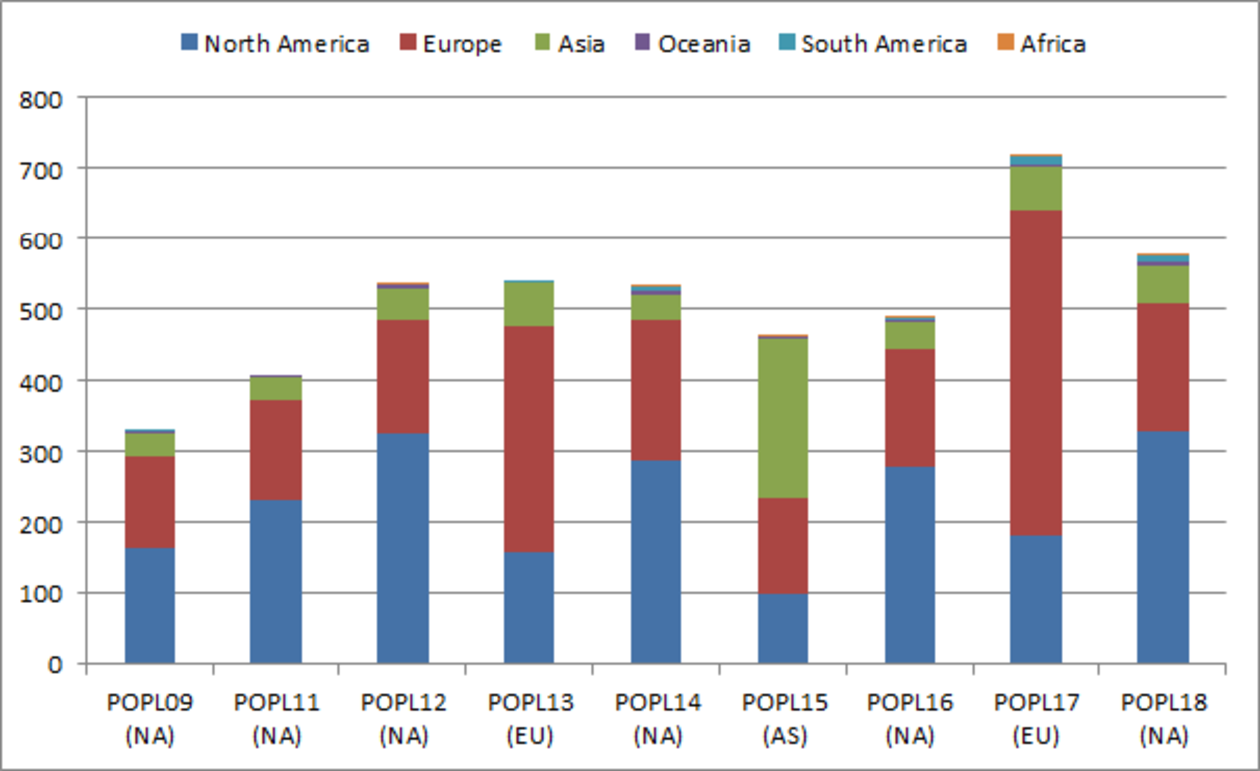
\includegraphics[width=0.45\textwidth,height=1.8in]{ParticipantsOriginPOPL.pdf}
  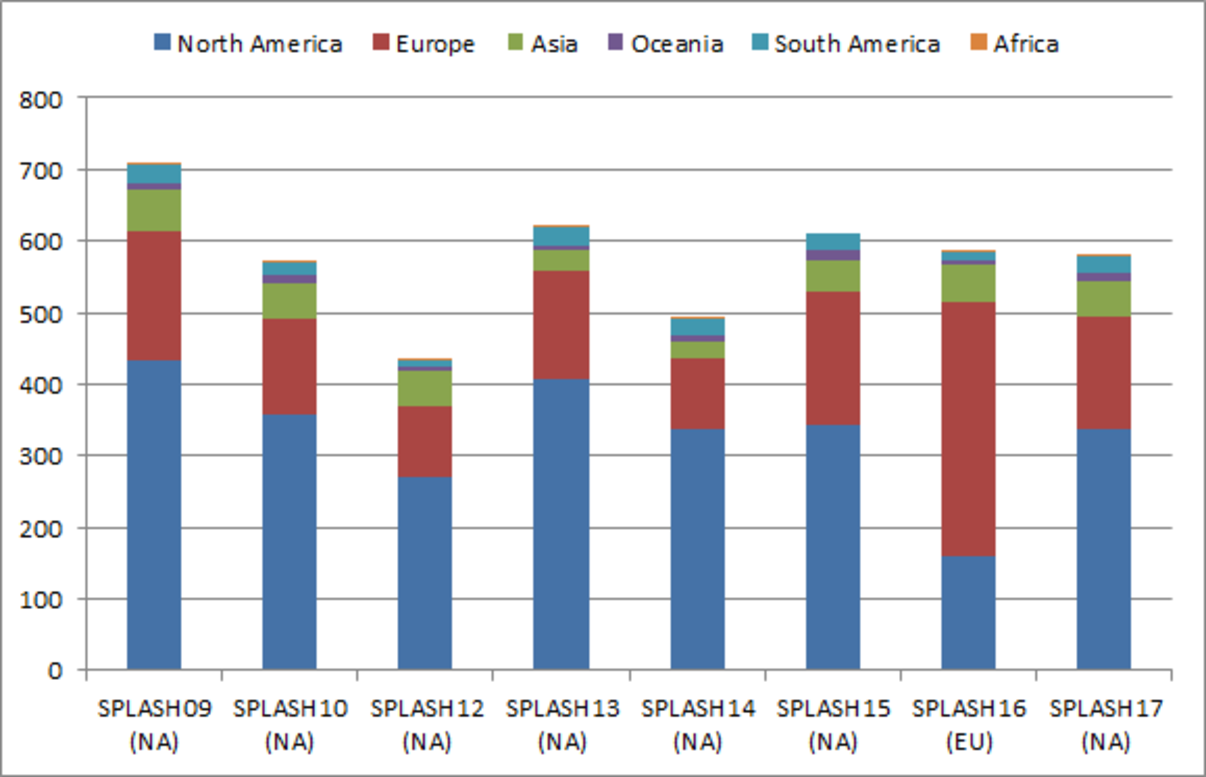
\includegraphics[width=0.45\textwidth,height=1.8in]{ParticipantsOriginSPLASH.pdf}
  \caption{Origin of participants for each conference, detail.}
  \label{fig:demo-per-event}
\end{figure}

This overall picture, however, hides some interesting facts pertaining to the
relationship between the conferences' locations and the origin of the participants.
Indeed, aggregating the attendance per conference intrinsically rests upon the
assumption of a uniform community attending each instance of the conference
every year. Table~\ref{fig:demo-per-event} and Figure~\ref{fig:demo-per-event}
show a more detailed breakdown of the origin of participants for each
conference, showing also the geographic region where the conferences were held.

These charts make it clear that the location of the conferences had a
substantial effect on attracting people from the same geographic areas. That
effect is quite visible for ICFP and POPL, with noticeable ups and downs of
the colored bars between North American and European participants when the
conferences were located in North America and Europe, respectively. Most
strikingly, Asian participation during POPL '15, ICFP '11 and ICFP '16,
events that took place on the Asian continent, is significantly higher than
usual: there appears to be a strong locality phenomenon. Crossing this data
with Table~\ref{table:footprint}, one can also notice that the only time
SPLASH took place in Europe turned out to be the least carbon-intensive
edition, challenging our previous observation that the conference appears to
be mostly North-America-centric.

\begin{table}
  \csvautotabular{../../output/sigplan/demographic_delta.csv}
\caption{Geographical distribution of participation conditioned by the location of the \event}
\label{table:local_effect}
\end{table}

Table~\ref{table:local_effect} attempts to measure this locality effect. The
table depicts, all conferences being considered at once, the geographical
distribution of attendance conditioned by the geographical location of the
\event. The Asian phenomenon previously hinted at is here extremely
apparent: while overall on average, 10.9\% of the participants come from Asia,
this number is roughly multiplied by a factor 4 when the \event takes place in Asia --
without any significant drop in total volume of attendance that could indirectly bump
the percentage.
But interestingly, this phenomenon also exists in the case of Europe (+22.29\%
deviation to the average) and North America (+12.15\% deviation to the average).
Despite their name, international conferences appear to exhibit a fairly strong
local component.

Overall, this data shows that the goal of geographic inclusion was,
indeed, accomplished by organizing the conferences in diverse geographic areas
of the world. It also places Figure~\ref{fig:demo-per-event} into a broader context:
a naive interpretation of that chart might lead us to conclude that North
America and Europe are where most of this community is, but it is not that
simple. Because of the regional effect on participation, the distribution of
participants also reflects the fact that most of these conferences were held in
North America and Europe (30), only a few were held in Asia (3), and none was
held in South America, Oceania, or Africa.

The situation may be summed up in two elementary observations:
\begin{obs}
  The vast majority of participants are split between North America and Europe,
  Asia to a much lesser degree. SPLASH and PLDI are strongly anchored in North
  America, ICFP and POPL fairly equally split between North America and Europe.
  \label{obs:dist-naive}
\end{obs}
This distribution, however, is \emph{strongly} dependent on the
location of the \event.
\begin{obs}
  There is a major ``locality" effect: it is both true that locality attract
  new participants, and distance repels some participants.
  \label{obs:locality}
\end{obs}

\subsection{How Often Did Participants Attend These Conferences?}
\label{subsec:overlap}

Section~\ref{subsec:demo}, through the study of the demographic distribution of
attendance, has suggested the existence of local communities that only
partake in conferences when they take place close to their place of residency.
One can conversely look for groups of regular attendees, that participate to a given \conf
regardless of the location it is held in.

\begin{figure}
  \centering
  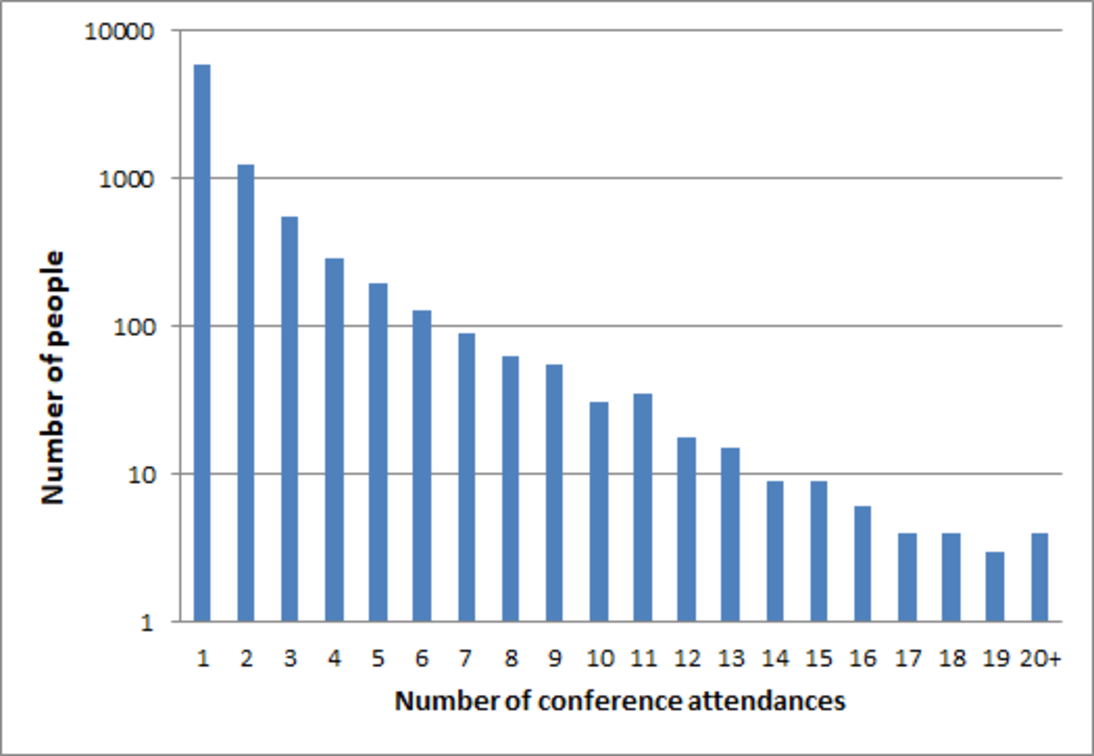
\includegraphics[width=0.6\textwidth]{AttendanceHist.pdf}
  \caption{Histogram of attendance.}
  \label{fig:hist_attendance}
\end{figure}

\begin{figure}
  \centering
  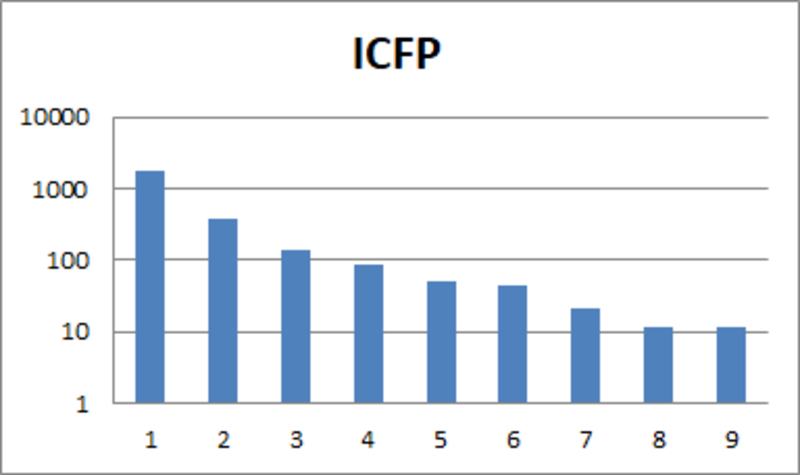
\includegraphics[width=0.45\textwidth,height=1.5in]{AttendanceHistICFP.pdf}
  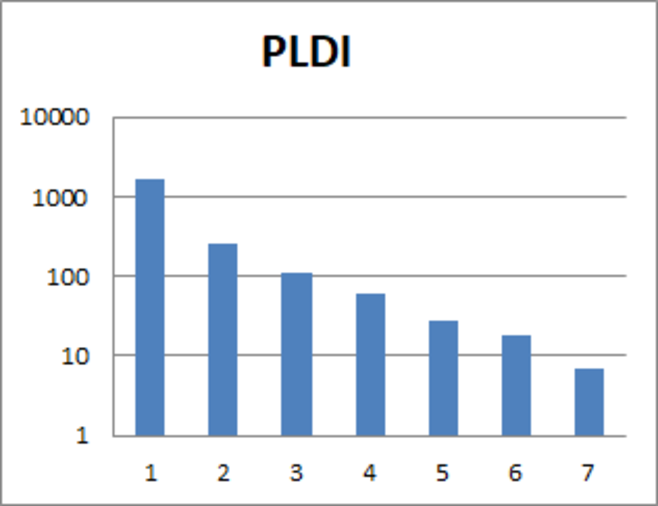
\includegraphics[width=0.4\textwidth,height=1.5in]{AttendanceHistPLDI.pdf}
  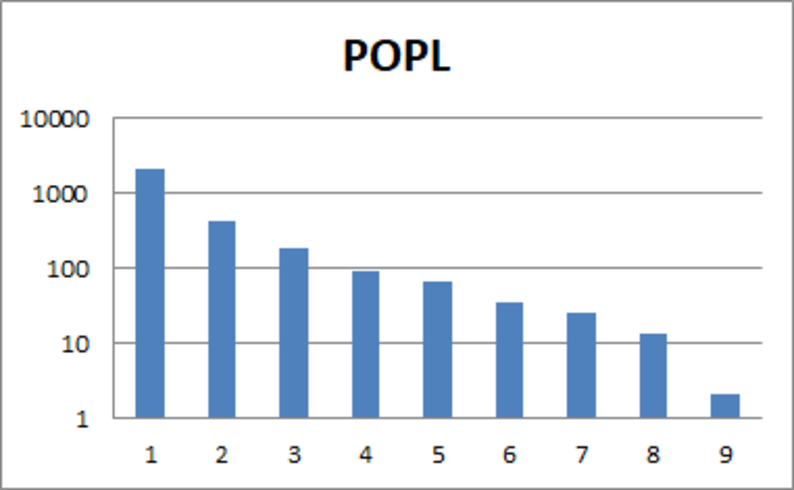
\includegraphics[width=0.45\textwidth,height=1.5in]{AttendanceHistPOPL.pdf}
  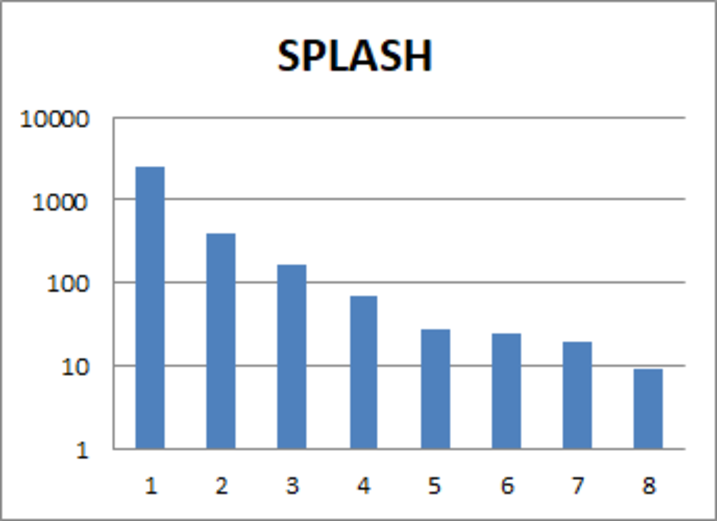
\includegraphics[width=0.4\textwidth,height=1.5in]{AttendanceHistSPLASH.pdf}
  \caption{Histogram of attendance for each conference series.}
  \label{fig:hist_attendance_per_conference}
\end{figure}

Figure~\ref{fig:hist_attendance} shows how often the same participants attended
multiple conferences. At the extremes, 6,009 people (69\%) attended only 1
conference, and 4 people attended 20 or more conferences. Participation is
dominated by single-conference participants, perhaps reflecting a large and
transient student population. The pattern is similar for each conference series,
shown in Figure~\ref{fig:hist_attendance_per_conference}.


\subsection{What Was the Participation Overlap Between These Conferences?}

We now take a closer look at the habits of these recurring participants.

\begin{table}
  \centering
  \begin{subtable}[b]{0.3\textwidth}
    \centering
    \csvautotabular{../../output/sigplan/overlap_cross_conf_ICFP_POPL.csv}
    \caption{POPL and ICFP}
  \end{subtable}
  \begin{subtable}[b]{0.3\textwidth}
    \centering
    \csvautotabular{../../output/sigplan/overlap_cross_conf_POPL_PLDI.csv}
    \caption{POPL and PLDI}
  \end{subtable}
  \begin{subtable}[b]{0.3\textwidth}
    \centering
    \csvautotabular{../../output/sigplan/overlap_cross_conf_POPL_SPLASH.csv}
    \caption{POPL and SPLASH}
  \end{subtable}
  \begin{subtable}[b]{0.3\textwidth}
    \centering
    \csvautotabular{../../output/sigplan/overlap_cross_conf_ICFP_PLDI.csv}
    \caption{ICFP and PLDI}
  \end{subtable}
  \begin{subtable}[b]{0.3\textwidth}
    \centering
    \csvautotabular{../../output/sigplan/overlap_cross_conf_ICFP_SPLASH.csv}
    \caption{ICFP and SPLASH}
  \end{subtable}
  \begin{subtable}[b]{0.3\textwidth}
    \centering
    \csvautotabular{../../output/sigplan/overlap_cross_conf_PLDI_SPLASH.csv}
    \caption{PLDI and SPLASH}
  \end{subtable}
   \caption{For every year, overlap in attendance between the events of two
     different conferences. The ``Any'' row depicts the percentage of unique
     participants that went at least once to both conferences over the available
     years of data.}
  \label{table:overlap-cross}
\end{table}

A first natural question is to ponder whether there is a significant overlap
in participation between conferences.
Table~\ref{table:overlap-cross} depicts, for each pairing of the four
conferences, the percentage of overlap. This measure is strikingly
low for most conferences.

\begin{obs}
  Cross-conference overlap is low: the tightest pairing sees slightly over 10\%
  of common attendance for a given year. Extending the overlap among any two years,
  the tightest pairing still sees less than a quarter of unique participants having
  participated at least once in both conferences.
  \label{obs:overlap-cross}
\end{obs}

%% \begin{table}
%% \centering
%%      \begin{subtable}[b]{0.4\textwidth}
%%        \centering
%%        \csvautotabular{../../output/sigplan/overlap_intra_conf_POPL.csv}
%%        \caption{Case of POPL}
%%      \end{subtable}
%%      \hfill
%%      \begin{subtable}[b]{0.4\textwidth}
%%        \centering
%%        \csvautotabular{../../output/sigplan/overlap_intra_conf_ICFP.csv}
%%        \caption{Case of ICFP}
%%     \end{subtable}

%%      \caption{For any two years, percentage of overlap in attendance at the corresponding editions of a conference (part 1)}
%%      \label{table:overlap-conf-alpha}
%% \end{table}

%% \begin{table}
%% \centering
%%      \begin{subtable}[b]{0.4\textwidth}
%%        \centering
%%        \csvautotabular{../../output/sigplan/overlap_intra_conf_PLDI.csv}
%%        \caption{Case of PLDI}
%%      \end{subtable}
%%      \begin{subtable}[b]{0.4\textwidth}
%%        \centering
%%        \csvautotabular{../../output/sigplan/overlap_intra_conf_SPLASH.csv}
%%        \caption{Case of SPLASH}
%%      \end{subtable}

%%      \caption{For any two years, percentage of overlap in attendance at the corresponding editions of a conference (part 2)}
%%      \label{table:overlap-conf-beta}
%% \end{table}

\begin{figure}
  \centering
  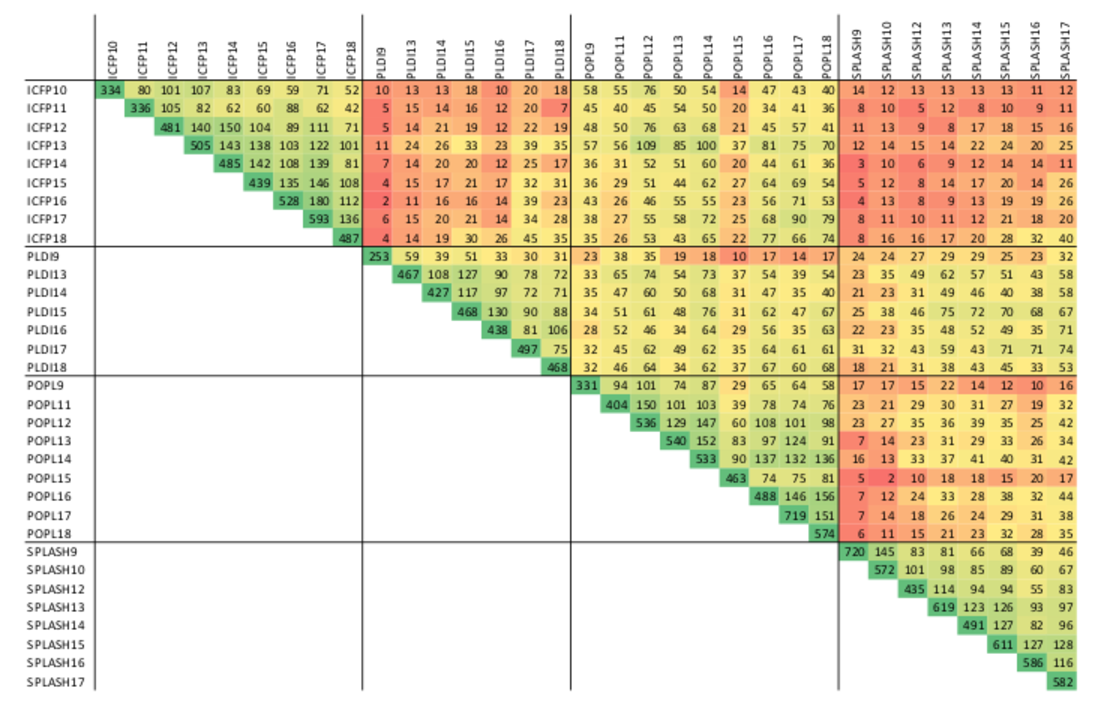
\includegraphics[width=\textwidth]{OverlapAnalysis-crop.pdf}
  \caption{Conference participation overlap.}
  \label{fig:overlap}
\end{figure}

Conversely, one can estimate the overlap for a given conference over time: for a
given conference at a time, and for any pair of years, compute the percentage of
attendees that participated in both events. This new information, as well as
the essential of Table~\ref{table:overlap-cross}, is synthesized graphically on
Figure~\ref{fig:overlap}.
With this bird-eye view of the permanence vs. transience of the
participants over time in SIGPLAN conferences, we can make a second observation,
temporal this time:

\begin{obs}
Temporal overlap is moderate: roughly a quarter of attendees at a given
conference were also present the year before at the same conference.
  \label{obs:overlap-temp}
\end{obs}

In principle, it is desirable to have a balance between repeat participants and
newcomers. Communities that don't attract new participants tend to stagnate; but
communities that don't have a core of repeat participants tend to lose focus.

The existence of a certain community associated with each conference series that
tends to repeat participation is clearly visible on the diagonal in
Figure~\ref{fig:overlap}. The highest overlap of all in particular was between
ICFP'16 and ICFP'17, with 180 repeaters. The four conference series show a
healthy balance between repeat participation and newcomers.

The weaker overlap between conferences in different series is also apparent.
For example, there is a somewhat surprising overlap between PLDI and
POPL, followed by ICFP and POPL and by PLDI and SPLASH. The weakest overlaps are
between ICFP and SPLASH, followed by ICFP and PLDI, and by POPL and SPLASH. It
is unclear whether the overlap, or lack thereof, between these conference series
is due to intellectual reasons or due to their dates. PLDI and POPL is the pair
that is most distant in time, typically June and January, respectively. ICFP and
SPLASH is the pair that is the closest in time, typically September and October.
Time proximity may detract cross-participation.

\begin{table}
  \csvautotabular{../../output/sigplan/number_of_participations.csv}
\caption{Overall and for each conference, the average number of instances a
  participant has taken part of, and the percentage of them that has
  attended at least $k$ instances, for $k\in\llbracket 2 \dots 5
  \rrbracket$. Remark: the means and percentages are here computed with
  respect to \emph{unique} participants.}
\label{table:recurrent}
\end{table}

\begin{table}
  \centering
  \begin{subtable}[b]{0.4\textwidth}
    \centering
    \csvautotabular{../../output/sigplan/old_timer_POPL.csv}
    \caption{Case of POPL}
  \end{subtable}
  \begin{subtable}[b]{0.4\textwidth}
    \centering
    \csvautotabular{../../output/sigplan/old_timer_ICFP.csv}
    \caption{Case of ICFP}
  \end{subtable}
  \\
  \begin{subtable}[b]{0.4\textwidth}
    \centering
    \csvautotabular{../../output/sigplan/old_timer_PLDI.csv}
    \caption{Case of PLDI}
  \end{subtable}
  \begin{subtable}[b]{0.4\textwidth}
    \centering
    \csvautotabular{../../output/sigplan/old_timer_SPLASH.csv}
    \caption{Case of SPLASH}
  \end{subtable}
  \caption{For each conference, percentage of participants that have been
    part of a previous edition of the same conference}
  \label{table:old-timers}
\end{table}

Finally, Table~\ref{table:recurrent} and \ref{table:old-timers} offer two
different views on recurrent participation. Table~\ref{table:recurrent}
represents respectively for the whole dataset (row ``ALL'') and for each
conference individually the average number of editions a participant has
been part of, as well as the percentage of participants that have been part
of at least a given number of editions of a conference. One striking fact is
that no less than 75\% of unique participants have been to just a single
edition.

Table~\ref{table:old-timers} is a normalization of the information represented
in Figure~\ref{fig:hist_attendance_per_conference}: for each instance of each
conference, it depicts the percentage of participants that have been part of a
previous instance of the conference (in our dataset).

\begin{obs}
Over all conferences, the average number of conferences a given participant
has attended is just 1.52. Less than 4\% of unique participants have been to
more than five events among our dataset.  Similarly, for any given \event,
more than half of the participants were experiencing this specific
conference for the first time.
  \label{obs:old-timers}
\end{obs}


\bcp{General question about all the pictures and tables: Are they
  consistent? (I.e., were the pictures generated from the data in the
  tables, or from earlier versions of that data?)}
\yz{Unfortunately no not at the moment: all tables are generated, but the Figures have been manually produced by Crista from her original take on the dataset. It would be great to regenerate them from the generated csv files, but I do not know how they have been generated exactly.}
